\newpage
\section{Abstract Factory Pattern}

Abstract Factory patterns work around a super-factory which creates other factories. This factory is also called as factory of factories. This type of design pattern comes under creational pattern as this pattern provides one of the best ways to create an object.
In Abstract Factory pattern an interface is responsible for creating a factory of related objects without explicitly specifying their classes. Each generated factory can give the objects as per the Factory pattern.

\subsection{Class Diagram}

\begin{figure}[h]
\centering
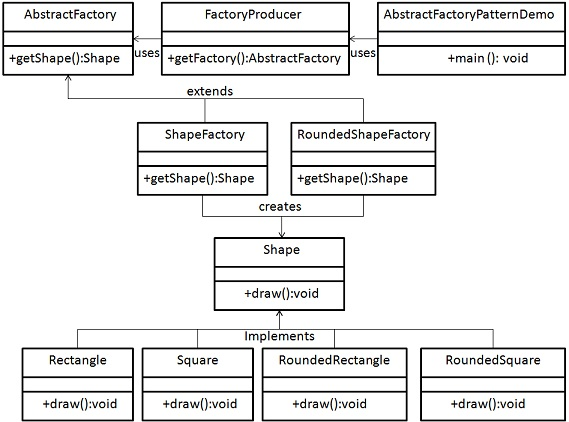
\includegraphics[scale=0.7]{abstractfactory}
\caption{Class Diagram of Abstract Factory Pattern}
\end{figure}

\newpage
\subsection{Source Code (Java)}
\subsubsection{Shape Interface}

\begin{minted}{java}
public interface Shape {
   void draw();
}
\end{minted}


\subsubsection{RoundedSquare Class}

\begin{minted}{java}
public class RoundedSquare implements Shape {
   @Override
   public void draw() {
      System.out.println("Inside RoundedSquare::draw() method.");
   }
}
\end{minted}

\subsubsection{RoundedRectangle Class}

\begin{minted}{java}
public class RoundedRectangle implements Shape {
   @Override
   public void draw() {
      System.out.println("Inside RoundedRectangle::draw() method.");
   }
}
\end{minted}

\subsubsection{Rectangle Class}

\begin{minted}{java}
public class Rectangle implements Shape {
   @Override
   public void draw() {
      System.out.println("Inside Rectangle::draw() method.");
   }
}
\end{minted}

\subsubsection{AbstractFactory abstract Class}

\begin{minted}{java}
public abstract class AbstractFactory {
   abstract Shape getShape(String shapeType) ;
}
\end{minted}

\subsubsection{ShapeFactory Class}

\begin{minted}{java}
public class ShapeFactory extends AbstractFactory {
   @Override
   public Shape getShape(String shapeType){    
      if(shapeType.equalsIgnoreCase("RECTANGLE")){
         return new Rectangle();         
      }else if(shapeType.equalsIgnoreCase("SQUARE")){
         return new Square();
      }	 
      return null;
   }
}
\end{minted}

\subsubsection{RoundedShapeFactory Class}

\begin{minted}{java}
public class RoundedShapeFactory extends AbstractFactory {
   @Override
   public Shape getShape(String shapeType){    
      if(shapeType.equalsIgnoreCase("RECTANGLE")){
         return new RoundedRectangle();         
      }else if(shapeType.equalsIgnoreCase("SQUARE")){
         return new RoundedSquare();
      }	 
      return null;
   }
}
\end{minted}

\subsubsection{FactoryProducer Class}

\begin{minted}{java}
public class FactoryProducer {
   public static AbstractFactory getFactory(boolean rounded){   
      if(rounded){
         return new RoundedShapeFactory();         
      }else{
         return new ShapeFactory();
      }
   }
}
\end{minted}

\subsubsection{Driver Class}

\begin{minted}{java}
public class AbstractFactoryDriver {
   public static void main(String[] args) {
      //get shape factory
      AbstractFactory shapeFactory = FactoryProducer.getFactory(false);
      //get an object of Shape Rectangle
      Shape shape1 = shapeFactory.getShape("RECTANGLE");
      //call draw method of Shape Rectangle
      shape1.draw();
      //get an object of Shape Square 
      Shape shape2 = shapeFactory.getShape("SQUARE");
      //call draw method of Shape Square
      shape2.draw();
      //get shape factory
      AbstractFactory shapeFactory1 = FactoryProducer.getFactory(true);
      //get an object of Shape Rectangle
      Shape shape3 = shapeFactory1.getShape("RECTANGLE");
      //call draw method of Shape Rectangle
      shape3.draw();
      //get an object of Shape Square 
      Shape shape4 = shapeFactory1.getShape("SQUARE");
      //call draw method of Shape Square
      shape4.draw();
      
   }
}
\end{minted}

\subsection{Output}

\begin{minted}{text}
Inside Rectangle::draw() method.
Inside Square::draw() method.
Inside RoundedRectangle::draw() method.
Inside RoundedSquare::draw() method.
\end{minted}